\documentclass{article}

\usepackage{hyperref}

% Below will configure hyperlink colors
\hypersetup{
    colorlinks=true,
    linkcolor=blue,
    filecolor=blue,
    urlcolor=blue,
}
\urlstyle{same}

\usepackage{enumitem}

% Below package is for precise positioning of images
\usepackage{float}
\usepackage{color}

% Below package is for syntax highlighted code
\usepackage{minted}
% Below set global setting fro minted package like line wraps and frame
\setminted{breaklines, frame=single}

% Below package is for including images
\usepackage{graphicx}
\usepackage[a4paper, inner=1.5cm, outer=3cm, top=2cm,bottom=3cm, bindingoffset=1cm]{geometry}
\setlength{\parskip}{.5em}

% The LaTeX graphics/graphicx package uses the first dot to find the extension. Package grffile changes this algorithm. This helps in including images files whose name contains more than 1 dot
\usepackage{grffile}


% Below package will create headings
%\pagestyle{headings}

% Below package will used to specify captions like "Figure 1: Nice Figure" in minipages using \captionof{figure}{Nice Figure}
\usepackage{caption}
\usepackage{hypcap} %This is needed for some warning in minipages


\begin{document}
\begin{titlepage}
   \vspace*{\stretch{1.0}}
   \begin{center}
      \Large\textsc{Signed/Unsigned Integer Arithmetic in C}\\
      \vspace{5mm}
      \Large\textit{Vineel Kovvuri}\\
      \url{http://vineelkovvuri.com}\\
   \end{center}
   \vspace*{\stretch{2.0}}
\end{titlepage}

\tableofcontents

\newpage
\section{Introduction}
This article is about understanding how integer conversions happen in C
language. C standard defines the integer conversion rules not specific to any
architecture. It makes things more complicated for the programmers to try and
understand them.

Why do we need integer conversions at all? The answer is simple we need to have
single type for the expression. Let's say we have an expression \textless
expr1\textgreater \textless op\textgreater \textless expr2\textgreater  when
expr1 and expr2 are different types, we want the resulting expression from this
to have one type.

The C99 specification below set of integer types called 'standard integer
types'. Interestingly, the sizes of these integer types are not defined at all.
It only defines the minimum supported size. For example, int need not be 8 bytes
long on x64 platforms, the only definition for int is it should have at least 16
bits and similarly long should have at least 32 bits it need not be 8 bytes
long. Depending on the platform and the processor architecture the ABI
(Application Binary Interface) and the 64bit programming model will define the
size of these basic types. Windows x64 follows LLP64(meaning only 'long long'
and pointer size is 64 bit wide), So below are the sizes of the standard types
that we are sticking to in this article.

\begin{center}
\begin{tabular}{|c|c|c|}
 Type       &Size       \\
 \hline
 signed char         & 1 bytes \\
 unsigned char       & 1 bytes \\
 signed short        & 2 bytes \\
 unsigned short      & 2 bytes \\
 signed int          & 4 bytes \\
 unsigned int        & 4 bytes \\
 signed long         & 4 bytes \\
 unsigned long       & 4 bytes \\
 signed long long    & 8 bytes \\
 unsigned long long  & 8 bytes
\end{tabular}
\end{center}

Also, The specification leaves other aspects of C language definition undefined
and this made room for optimization for the compilers. For example, the result
of signed arithmetic leading to overflow/underflow is not defined because the
specification predates to the machine architectures when 2's complement
representation for -ve numbers is not universal, Even though virtually every
architecture now uses 2's complement representation for -ve numbers. Hence the
result of unsigned overflow/underflow is well defined but not signed
overflow/underflow!

\section{How signed-ness is represented in the hardware?}
Processors do have the concept of signed/unsigned, but unlike in C language,
where this information is baked into the variable type definition, processor
registers do not hold this type information. After all, registers are just
placeholders data. But the instructions themselves have the notion of
signed/unsigned, That is why we have signed 'imul', unsigned 'mul', signed
(JL/JG) vs unsigned(JB/JA) jump instructions. This is an important distinction
between programming languages and machine code. It helps in understanding how
high-level code gets translated to underlying machine code. Instructions which
produce/consume signed data understand that -ve numbers should be in 2's
complement form. So if a register (8bit) has 11110110 it's up to the instruction
to treat that data as either -10 (signed) or 246 (unsigned). If an operation
results in a -ve result say -5 then destination register will be written
11111011(2's complement representation of -5). 'add' and 'sub' instructions
themselves are not affected by signed and unsigned numbers because of modulo
arithmetic.

\section{How signed-ness is interpreted in assembly?}
In one of the above paragraphs, we said, processor registers does not hold any
signed/unsigned type information with them and it's up to the instructions to
interpret the data as either signed or unsigned. But the interesting thing
about x86/x64 processors is they provide a flag register where some of the
bits are called Status Flags. These bits represent the specific effect of
what happened with the previous instruction.

The most important flags of these for our discussion are

\begin{enumerate}[noitemsep]
    \item Carry flag - Set if an arithmetic operation generates a carry or a borrow out of the most-
significant bit of the result; cleared otherwise. \textbf{This flag indicates
an overflow condition for unsigned-integer arithmetic}.
    \item Sign flag - Set equal to the most significant bit of the result, which is the sign bit of a signed
integer. (0 indicates a positive value and 1 indicates a negative value.)
    \item Overflow flag - Set if the integer result is \textbf{too large a
    positive number or too small a negative number (excluding the sign-bit) to
    fit in the destination operand} cleared otherwise. This flag
indicates an overflow condition for signed-integer (two's complement) arithmetic
\end{enumerate}

Of the above three status flags, Carry flag is obvious but other two flags need
some explanation. Sign flag is set irrespective of whether you are treating the
numbers as positive or negative, All it cares is if the result's MSB is set or
not.

For example in below code, 'sub' can treat 0x81 as -127 or +129. So the result
can also be either interpreted as -128 or +128, But the processor after
executing 'sub' it indicates this possibility in Sign Flag. So operations(JA/JB)
who want to treat the result an unsigned will ignore this sign flag whereas
operations (like JG/JL) who treat it as signed will take this sign flag into
account.
\begin{minted}{asm}
    mov al, 0x81
    sub al, 0x1     // This triggers sign flag
\end{minted}

Overflow flag is a little different. First of all, the Overflow flag is not set
when an operation results in an overflow of the number that can be represented
in a register. Like for example, if we try to add 1 to 0xff does not set this
bit.
\begin{minted}{asm}
    mov al, 0xFF // 0b11111111
    add al, 0x1  // This will not trigger Overflow flag
\end{minted}
Overflow flag is mainly meant for indicating if there is a chance of result if
interpreted as signed will cross beyond what can be represented in the register.
for example if we take a byte(al) it can contain value from 0b00000000(0) to
0b11111111(255) as unsigned or 0b10000000(-128) to 0b00000000(0) and 0b01111111
(127) as signed number. Now overflow flag is set when a result goes beyond
0b01111111 i.e., too large a positive number and less than 0b10000000 i.e., too
small a negative number

\begin{minted}{asm}
    mov al, 0x7e // This is always positive
    add al, 0x2  // This will trigger overflow flag
\end{minted}

Let us see how overflow flag is used to determine the below conditional when
var1 and var2 are signed numbers.
\begin{minted}{c}
    if (var1 < var2) {
        printf("var1 < var2");
    }
\end{minted}
you find var1 \textless var2 we calculate var1-var2 the result should be -ve
meaning sign flag should be set b ut what if we are

if condition is implemented as jl instruction of a prior cmp instruction. But
this jl say execute printf if SF != OF, for the subtraction var1 - var2 to hold
true alway var1 should be smaller than var2 but because cmp is nothing but sub
instruction which substracts var2 from var1 there couple of cases that araises.
\begin{minted}[escapeinside=||]{text}
var1 = -125;
var2 = 10;
var1-var2 => -135 => |\bf{which cannot be represented in a byte meaning the sign
bit of the byte will not be set but the overflow bit gets set. So SF=0 and
OF=1}|

var1 = -120;
var2 = -100;
var1-var2 => -20 => |\bf{this can be represented in a byte and its -ve so SF = 1
but because it is still under the range of singed numbers representable in a
byte OF = 0}|
\end{minted}
That is why jl is defined as SF != OF, When this is true it means var1 < var2
even if var1 and var2 are signed(meaning -ve numbers)

\section{Signed vs Unsigned integers in C}
Signed numbers are the way -ve numbers are represented and unsigned numbers are
the way in which +ve numbers are represented. If let's say a data type has 1
byte of storage then the possible bit representation will be from  0b00000000(0)
- 0b11111111(255). Now, these 255 valid slots can be interpreted as all positive
numbers or divide the range into two halves and call one half of the slot as
positive and other as negative numbers. There are other alternate representations
for -ve number but almost all systems use 2's complement notation to represent
-ve numbers. The take away here is if we include -ve number in the 255 slots
then we will represent from -128 to 127. According to 2's complement notation
-128 is represented as 0b10000000(0x80) whereas 127 is represented as 0b01111111
(0x7F).

\section{Integer Arithmetic Conversions in C}
C language defines below set of rules to convert the arguments in an expression.

\subsection{Rank}
Every integer type has an integer conversion rank defined as follows:
\begin{enumerate}[noitemsep]
    \item No two signed integer types shall have the same rank, even if they
    have the same representation.
    \item The rank of a signed integer type shall be greater than the rank of any signed integer
    type with less precision.
    \item The rank of long long int shall be greater than the rank of long int, which
    shall be greater than the rank of int, which shall be greater than the rank of short
    int, which shall be greater than the rank of signed char.
    \item The rank of any unsigned integer type shall equal the rank of the corresponding
    signed integer type, if any.
    \item The rank of any standard integer type shall be greater than the rank of any extended
    integer type with the same width.
    \item The rank of char shall equal the rank of signed char and unsigned char.
    \item The rank of \_Bool shall be less than the rank of all other standard integer types.
    \item The rank of any enumerated type shall equal the rank of the compatible integer type
    (see 6.7.2.2).
    \item The rank of any extended signed integer type relative to another extended signed
    integer type with the same precision is implementation-defined, but still subject to the
    other rules for determining the integer conversion rank.
    \item For all integer types T1, T2, and T3, if T1 has greater rank than T2 and T2 has
    greater rank than T3, then T1 has greater rank than T3.
\end{enumerate}
At a high level the gist of above rules is as follows
\begin{minted}{text}
 Rank(signed char) ==  Rank(unsigned char) <  Rank(signed short) ==  Rank(unsigned short) <  Rank(signed int) ==  Rank(unsigned int) <  Rank(signed long) ==  Rank(unsigned long) <  Rank(signed long long) ==  Rank(unsigned long long)
\end{minted}

\subsection{Integer Promotions}
    The following may be used in an expression wherever an int or unsigned int may
    be used:
    \begin{itemize}[noitemsep]
        \item An object or expression with an integer type whose integer conversion rank is less
        than or equal to the rank of int and unsigned int.
        \item A bit-field of type \_Bool, int, signed int, or unsigned int.
    \end{itemize}
\begin{itemize}[noitemsep]
    \item 1a) If an int can represent all values of the original type, the value is converted to an int;
    \item 1b) otherwise, it is converted to an unsigned int.
    These are called the integer promotions. All other types are unchanged by the integer promotions.
\end{itemize}

\subsection{Usual arithmetic conversions}
\begin{itemize}[noitemsep]
    \item 2a) If both operands have the same type, then no further conversion is needed.

    \item 2b) Otherwise, if both operands have signed integer types or both have unsigned
    integer types, the operand with the type of lesser integer conversion rank is
    converted to the type of the operand with greater rank.

    \item 2c) Otherwise, if the operand that has unsigned integer type has rank greater or
    equal to the rank of the type of the other operand, then the operand with
    signed integer type is converted to the type of the operand with unsigned
    integer type.

    \item 2d) Otherwise, if the type of the operand with signed integer type can represent
    all of the values of the type of the operand with unsigned integer type, then
    the operand with unsigned integer type is converted to the type of the
    operand with a signed integer type.

    \item 2e) Otherwise, both operands are converted to the unsigned integer type
    corresponding to the type of the operand with signed integer type.
\end{itemize}

\subsubsection{Rule 2c interpretation}
The gist of 2c is to make sense of
expressions like z = a+b where a is singed number and b is unsigned number. Now
a 4 byte signed int is added to 8 byte unsigned long long, according
to this rule 4 byte signed int will become 8 byte unsigned long long. The
important point to remember here is conversion of signed int to unsigned long
long, The way the compiler does this is by sign extend 4 byte signed number so
that its absolute value will not change i.e.., -10 remain -10 whether it is a 4
byte or 8 byte. But according to these rules the expression will have the type
unsigned long long so statements like below will result in unexpected behavior.
Since the var1+var2 is an unsigned expression the compiler will enforce it by
using a unsigned jump instruction called jae instead of jge instruction.

Whenever a signed data type has to be converted to unsigned data type the
absolute value remains unchanged because of sign extension will be done using
movsx instruction. So if a variable is type signed short with value -10, when
this variable is sign extended to unsigned int the value of even after the
conversion remains -10 when interpreted as singed int because the binary
represent for -10 for 2 byte storage and 4 byte storage yields the same.

\begin{figure}[H]
\centering
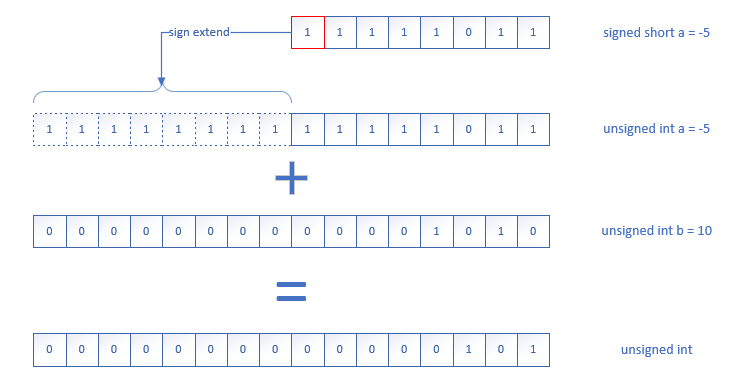
\includegraphics[width=\textwidth]{signed-short-to-unsigned-int.png}
\caption{signed number converted to unsigned numbers}
\end{figure}

\href{https://godbolt.org/}{godbolt's compiler explorer} is very helpful in
understanding how the compiler translates expressions and apply the above rules.
Clang AST view especially helps in graphically looking at how these
promotions/conversion happen

\begin{minted}{c}
signed int var1 = -100;
unsigned long long var2 = 10;
if (var1 + var2 < 0) { //resulting unsigned long long expression will never be lessthan 0
    printf("This will never get printed");
}
\end{minted}
\begin{minted}{asm}
$LN4:
        sub     rsp, 56                             ; 00000038H
        mov     DWORD PTR var1$[rsp], -100                ; ffffffffffffff9cH
        mov     QWORD PTR var2$[rsp], 10
        movsxd  rax, DWORD PTR var1$[rsp]
        add     rax, QWORD PTR var2$[rsp]
        test    rax, rax
        jae     SHORT $LN2@main      //This is an unsigned jump
        lea     rcx, OFFSET FLAT:$SG4416
        call    printf
$LN2@main:
        xor     eax, eax
        add     rsp, 56                             ; 00000038H
        ret     0
main    ENDP
\end{minted}
\begin{minted}{text}
Fragment of clang's AST for above program

      |-BinaryOperator <line:7:9, col:23> 'bool' '<'
      | |-BinaryOperator <col:9, col:16> 'unsigned long long' '+'
      | | |-ImplicitCastExpr <col:9> 'unsigned long long' <IntegralCast>
      | | | `-ImplicitCastExpr <col:9> 'int' <LValueToRValue>
      | | |   `-DeclRefExpr <col:9> 'int' lvalue Var 0x55ea65e030e0 'var1' 'int'
      | | `-ImplicitCastExpr <col:16> 'unsigned long long' <LValueToRValue>
      | |   `-DeclRefExpr <col:16> 'unsigned long long' lvalue Var 0x55ea65e031b0 'var2' 'unsigned long long'
      | `-ImplicitCastExpr <col:23> 'unsigned long long' <IntegralCast>
      |   `-IntegerLiteral <col:23> 'int' 0
\end{minted}


These rules can only dictate what need to be done for each expression in a
statement one at a time. It cannot determine the type of the complete
statement at once because of this we might end up with unexpected results if
we are not careful enough about how the type is propagating.
for example,in var = exp1 + exp2*exp3 the rules can only tell how exp2*exp3
interact and how that result interacts with exp1. exp2*exp3's new type may not
gel well with exp1 and might result in an unexpected result.

\subsubsection{Rule 2d interpretation}
Rule 2d tries to make sense when you have two variables with small
the unsigned number and signed number are present in an expression and the
singed storage can hold the unsigned number entirely, then by this
rule, the unsigned number gets converted to signed number.


\begin{figure}[H]
\centering
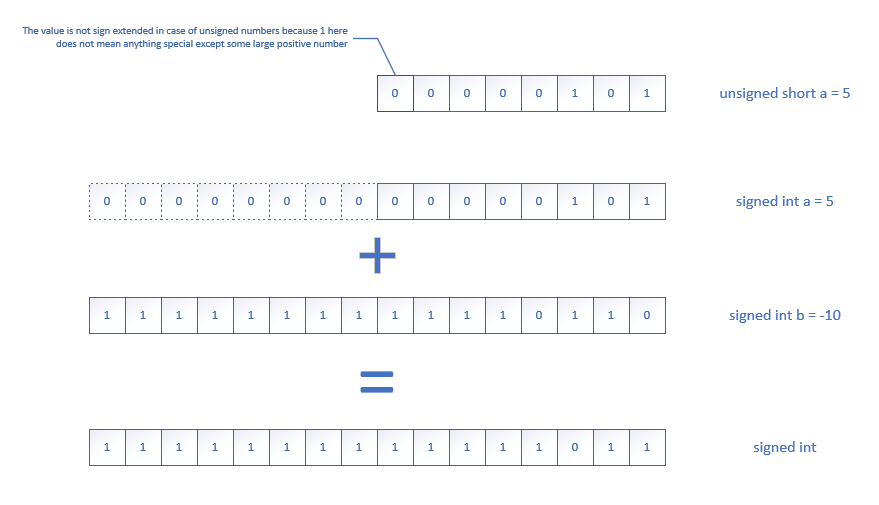
\includegraphics[width=\textwidth]{unsigned-short-to-signed-int.png}
\caption{unsigned number converted to signed numbers}
\end{figure}

For example:
\begin{minted}{c}
unsigned int var1 = 100;
signed long long var2 = -10;
if (var1 + var2 < 0) { //resulting in signed long long expression
    printf("This gets printed if var1 + var2 is < 0");
}
\end{minted}
\begin{minted}{asm}
        sub     rsp, 56                             ; 00000038H
        mov     DWORD PTR var1$[rsp], 100   ; 00000064H
        mov     QWORD PTR var2$[rsp], -10
        mov     eax, DWORD PTR var1$[rsp]
        add     rax, QWORD PTR var2$[rsp]
        test    rax, rax
        jge     SHORT $LN2@main                // This is a signed jump
        lea     rcx, OFFSET FLAT:$SG4869
        call    printf
$LN2@main:
        xor     eax, eax
        add     rsp, 56                             ; 00000038H
        ret     0
main    ENDP
\end{minted}
\begin{minted}{text}
Fragment of clang's AST for above program

      |-BinaryOperator <line:7:9, col:23> 'bool' '<'
      | |-BinaryOperator <col:9, col:16> 'long long' '+'
      | | |-ImplicitCastExpr <col:9> 'long long' <IntegralCast>
      | | | `-ImplicitCastExpr <col:9> 'unsigned int' <LValueToRValue>
      | | |   `-DeclRefExpr <col:9> 'unsigned int' lvalue Var 0x56305e1200e0 'var1' 'unsigned int'
      | | `-ImplicitCastExpr <col:16> 'long long' <LValueToRValue>
      | |   `-DeclRefExpr <col:16> 'long long' lvalue Var 0x56305e1201a8 'var2' 'long long'
      | `-ImplicitCastExpr <col:23> 'long long' <IntegralCast>
      |   `-IntegerLiteral <col:23> 'int' 0
\end{minted}

\subsubsection{Rule 2e interpretation}
And finally, Rule 2e is applied only between unsigned int and signed long
because neither 2c,2d fits these type on LLP64 model. One interesting thing we
can observe if read between the lines is, the resultant type has unsignedness
but the type is of signed variable and also both operand types are converted
unlike other rules.
For example:
\begin{minted}{c}
unsigned int var1 = 100; // this gets converted to unsigned long
signed long var2 = -10;  // this will also converted to unsigned long
if (var1 + var2 < 0) { //resulting type is unsigned long
    printf("This will not be printed");
}
\end{minted}
\begin{minted}{asm}
        sub     rsp, 56                             ; 00000038H
        mov     DWORD PTR var1$[rsp], 100   ; 00000064H
        mov     DWORD PTR var2$[rsp], -10
        mov     eax, DWORD PTR var2$[rsp]
        mov     ecx, DWORD PTR var1$[rsp]
        add     ecx, eax
        mov     eax, ecx
        test    eax, eax
        jae     SHORT $LN2@main             // This is an unsigned jump
        lea     rcx, OFFSET FLAT:$SG4869
        call    printf
$LN2@main:
        xor     eax, eax
        add     rsp, 56                             ; 00000038H
        ret     0
main    ENDP
\end{minted}
\begin{minted}{text}
Fragment of clang's AST for above program

      |-BinaryOperator <line:7:9, col:23> 'bool' '<'
      | |-BinaryOperator <col:9, col:16> 'long' '+'
      | | |-ImplicitCastExpr <col:9> 'long' <IntegralCast>
      | | | `-ImplicitCastExpr <col:9> 'unsigned int' <LValueToRValue>
      | | |   `-DeclRefExpr <col:9> 'unsigned int' lvalue Var 0x564cedbd0100 'var1' 'unsigned int'
      | | `-ImplicitCastExpr <col:16> 'long' <LValueToRValue>
      | |   `-DeclRefExpr <col:16> 'long' lvalue Var 0x564cedbd01c8 'var2' 'long'
      | `-ImplicitCastExpr <col:23> 'long' <IntegralCast>
      |   `-IntegerLiteral <col:23> 'int' 0
\end{minted}

\subsection{Integer conversion matrix on LLP64 Programming Model}
Below table summaries the rules applied for each expression combination
\begin{figure}[H]
\centering
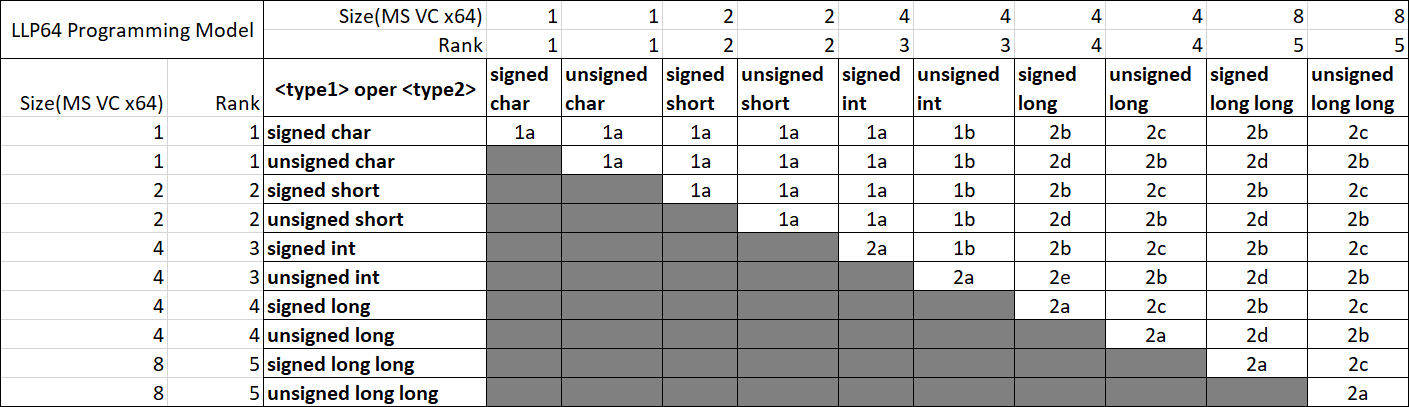
\includegraphics[width=\textwidth]{Integer-Arithmetic-All-Datatypes.png}
\caption{Rules applied for each combination of expression}
\end{figure}

Below table summaries the resulting data type of the expression
\begin{figure}[H]
\centering
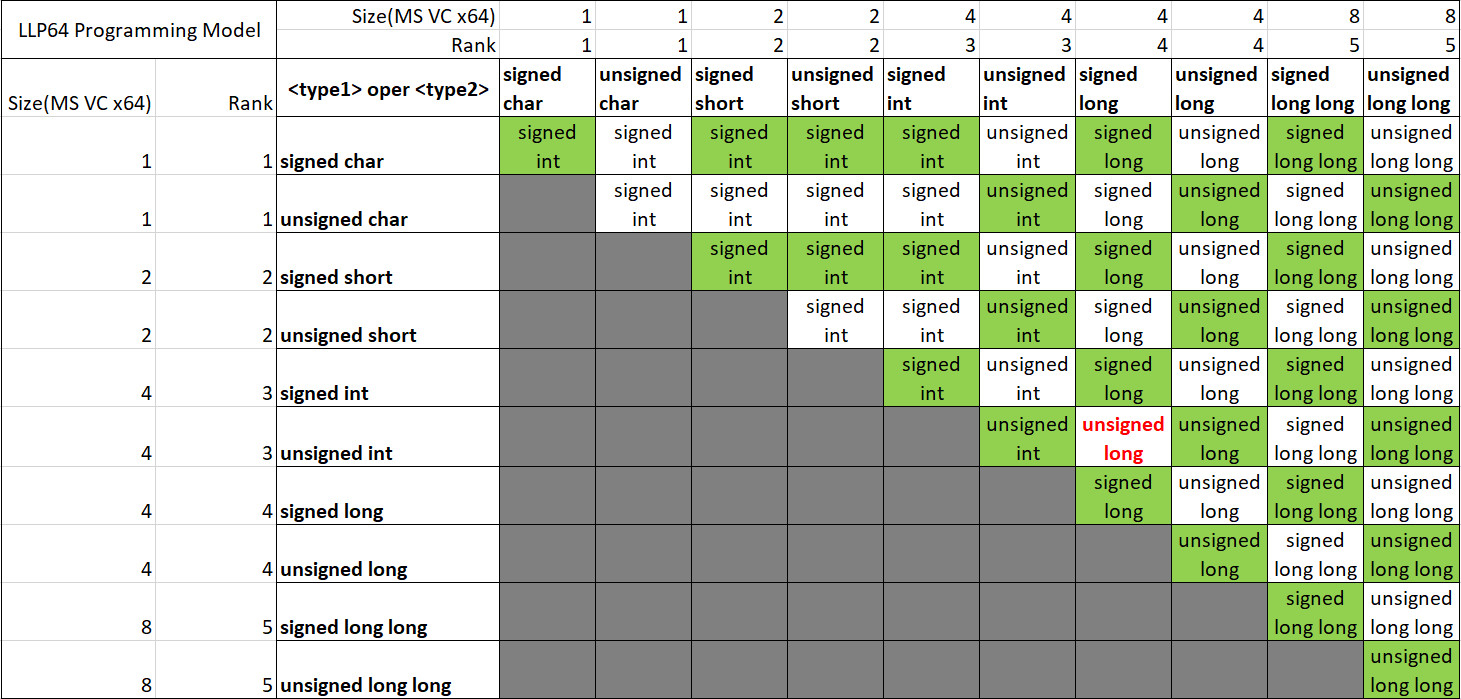
\includegraphics[width=\textwidth]{Resulting-Datatypes.png}
\caption{Resulting type of the expression}
\end{figure}


\section{References}
\begin{enumerate}[noitemsep]
\item \href{https://wiki.sei.cmu.edu/confluence/display/c/INT02-C.+Understand+integer+conversion+rules}{INT02-C. Understand integer conversion rules}
\item \href{http://www.open-std.org/jtc1/sc22/wg14/www/docs/n1256.pdf}{C99 Standard}
\item \href{http://blog.robertelder.org/signed-or-unsigned/}{Should I use Signed or Unsigned Ints In C? (Part 1)}
\item \href{http://blog.robertelder.org/signed-or-unsigned-part-2/}{Should I use Signed or Unsigned Ints In C? (Part 2)}
\item \href{http://ref.x86asm.net/coder-abc.html}{X86 Opcode and Instruction Reference}
\item \href{https://stackoverflow.com/a/42589535/2407966}{Why is imul used for multiplying unsigned numbers?}
\item \href{http://www.unix.org/version2/whatsnew/lp64_wp.html}{System V Application Binary Interface AMD64 Architecture Processor Supplement}
\item \href{https://software.intel.com/sites/default/files/article/402129/mpx-linux64-abi.pdf}{Why did the Win64 team choose the LLP64 model?}
\item \href{https://blogs.msdn.microsoft.com/oldnewthing/20050131-00/?p=36563}{Abstract Data Models}

\end{enumerate}

\end{document}